\documentclass[12pt]{article}
\usepackage[margin=3cm]{geometry}
\usepackage{enumitem}
\usepackage{listings}
\usepackage{graphicx}
\title{OS CS219 Notes}
\author{}
\date{\today}
\begin{document}
\maketitle
\setlength{\parskip}{6pt}
\setlength{\parindent}{0pt}
\section{Introduction}
\noindent An \textbf{OS}(operating system) alias \textbf{Master Control Program} alias \textbf{System software} is software than enables the user to access the hardware resources of a computer 
in a controlled manner. It acts as a layer of abstraction allowing the user to not worry
about hardware level access and just provides access to a few methods needed by the user


\noindent The OS has several uses/functions in a computer
\begin{itemize}[topsep=0pt, partopsep=0pt, itemsep=0pt, parsep=0pt]
    \item Manages resources as a single \textbf{central entity} and hence efficiently
    \item \textbf{Virtualizes} physical resources to be utilized by multiple processes\footnote{process is defined later}
    \item \textbf{Isolates} and protects processes from one another by not allowing direct access to hardware 
    \item Provides a set of system calls for the user to access hardware resources
    \item Starts processes and allocates and manages memory required by said process during execution
\end{itemize}

\noindent Thus it is easy to see that the OS has several important functions to perform inorder to enable an abstraction of hardware from the users

\section{Process and Virtualization}

\noindent A process is just the sequence of execution of instructions by the CPU
. When we write and compile a program it gets converted into a sequence of instructions whose first \textit{instruction address} is fed to the PC and as we know 
the sequence of instructions for that program starts getting executed one by one. This is called a process. So when we run a program a \textit{process} is created.


\subsection{Context switching}
\label{section:context}
How do we tell the CPU to start a process. First obviously we need to feed the address of the first instruction of the process to the \textbf{Program Counter}. We also need to set 
the stack pointer and other registers with appropriate values. This is called \textbf{setting up the context} for a process. This job is done by the OS 
.After the context is set the OS takes a back seat and allows the CPU to do its work


\noindent However this has a few issues. Firstly, when the process requests for data from say the hard drive there is a gap where the CPU 
is on standby which is wasteful since other processes also require it. Secondly, we also want responsiveness from our system ie when
we have a process running we also may want to interact with other processes. 


Both of these issues are solved by \textbf{concurrent} execution. Basically we run a process for a while and when the CPU is on standby or after a 
particular interval of time we save the \textit{context} (ie) states of all registers including PC and start the other process by setting up its context this repeats
for a while and eventually the partially executed process's context is set and it is continued.
This is reffered to as \textbf{context switching} and is an important part of Virtualization\footnote{Read further to know what it is} of the CPU.
Note that a part of the OS (ie) \textit{OS scheduler} decides which program to run at what time

\subsection{Virtualization}
Virtualization refers to the creation of an illusion that each of the processes have full access hardware resources\footnote{It is useful to think of Virtualization as the OS lying to each process about it having full access to a resource}. This
enables the hardware to act much more powerfully than they are capable of. For example, as mentioned above context switching creates the illusion
of the presence of multiple cores each assigned to one process whereas in reality it is just one core.
Infact this is refered to as \textbf{Hyperthreading}. Apart from the CPU memory, addresses can be virtualized.

\section{Memory allocation and Isolation}
\label{section:mem_alloc}
\subsection{Memory}
As we learnt in CS230, memory for a process/program is allocated as a fixed number of bytes. The inital bytes
of this memory is the instructions and the global/static variables. Local variables aren't initialised in memory since
we do not know the number of times each function is called, instead we have a dynamically growing stack whose starting address is
stored in the special \textit{stack pointer register}. This stack grows and shrinks as necessary functions are called and they return values.
\footnote{The structure used here is a stack since functions are inherently \textit{LIFO} functions called last return first}.


Apart from this we have a heap which can be accessed by user to store dynamically increasing data structures. We can request the
OS to allocate certain number of bytes and return a pointer to said bytes


Here again however the OS plays tricks on the processes. Since it is impractical for the OS to allocate to 
allocate memory for the process continguosly it allocates them in chunks but returns a \textbf{virtual address} (Recall Virtualization) to the program. This "virtual address" is the
address returned when the user requests the OS for an address of the data stored. Here again the OS lies to the process creating the illusion that it has access to continguos memory starting
from some location

\subsection{Isolation}
    Now we understand that the OS allows multiple processes to run at the same time and share resources
    But this raises a huge issue since processes are supposed to be independent and processes being to affect other 
    processes would cause problems. The OS takes care of this too by maintaing strict control over access to hardware

    The OS is the only entity with access to hardware and process can make specific requests to the OS to use hardware
    via \textit{system calls}\footnote{syscalls can't be accessed directly usually. They are in a language's standard library}. Infact there are two types of instructions and processer modes corresponding to them

    \begin{itemize}[topsep=0pt, partopsep=0pt, itemsep=0pt, parsep=0pt]
        \item \textbf{Privileged instructions} - special instructions that can interact with hardware. Generated by syscalls,device drivers
        CPU is in \textbf{kernel} mode while executing them 
        \item \textbf{Unprivileged instructions} - simple instructions that do not need access to hardware. Given by user processes. CPU is in \textbf{user} mode while running them
    \end{itemize}

    The CPU is always in user mode except the following cases.
    \begin{itemize}[topsep=0pt, partopsep=0pt, itemsep=0pt, parsep=0pt]
        \item A syscall is made
        \item Interrupt occurs
        \item Error needs to be handled 
        \item Context switching needs to happen for say concurrent running
    \end{itemize}
    
    Note that when a syscall is made the OS code pertaining to it is executed and then control is return back to user code
    \\\textbf{Interrupt:} In addition to running programs a CPU has to handle external inputs from devices like a mouse click.
    This is called an Interrupt. During an interrupt control is given to the OS(Kernel mode of CPU) which deals with the interrupt and returns
    control to the user process \footnote{This means saving context, handling the interrupt and setting context of the past status}


    \noindent\textbf{Device Driver:} I/O is managed by the device controller(Hardware) and device driver\\(software)\footnote{This is part of the OS}.
    The driver initializes IO devices and it starts IO operations like reading from the disk. It also handles the above mentioned interrupts


    \section{Process abstraction and attributes}

    As we have discussed above about a process it is a sequence of instructions running in the cpu.
    Also as discussed in section \ref{section:context} a process can run for a while, then be blocked and run again.
    Hence a process switches from one \textit{state} to another during its execution. We can note that this process state changes only when the kernel goes to user mode.\footnote{Since the change is done by the kernel's OS scheduler}

    \begin{figure}[h]
        \centering
        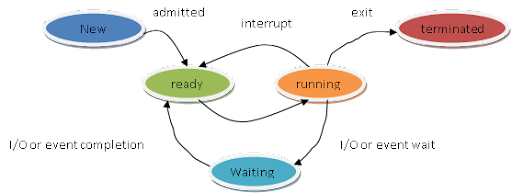
\includegraphics[width = 10cm]{process-state.png}
        \caption{Figure to show process state switching}
        \label{process-state}
    \end{figure}
    {\large A process is defined by several \textit{attributes} that define it:}
    \begin{itemize}[topsep=0pt, partopsep=0pt, itemsep=0pt, parsep=0pt]
        \item \textbf{PID}: Unique process identifier given to each process
        \item \textbf{PPID}: PID of a parent process\footnote{Parent discussed later}
        \item \textbf{Context}: Context is saved when switching happens. We have discussed what the context of a process refer \ref{section:context}
        \item \textbf{File descriptors}: A record of all the files open by a process is stored in form of pointers in 
        an array. Elements at index 0,1,2 refer to std input, std output and error files. As we open more files for
        a process a pointer to it is created and added to the end of the array. This poiner is what is returned as a 
        \textit{file descriptor} for the user to perform read or write operations.
        \item \textbf{State}: A process can be in 3 states
        \begin{enumerate}[topsep=0pt, partopsep=0pt, itemsep=0pt, parsep=0pt]
            \item \textbf{Running}: The CPU is currently executing instructions of the process
            \item \textbf{Blocked/suspended}: The process cannot run for a while. Maybe it requested data from drive and is waiting for its arrival
            \item \textbf{Ready/runnable}: Process can be run and is waiting for \textit{OS scheduler} to give it a CPU/core to use
        \end{enumerate}
        \item \textbf{Memory}: Each process uses/is allocated a fixed amount of memory by the OS and its locations are stored
        \item \textbf{Page Table}: The OS lies to the process about memory addresses(Virtual address \footnote{refer Section \ref{section:mem_alloc}}). The real address mapping to the corresponding
        virtual address is stored in the page table. The page table can be used to get the real address corresponding to each virtual address
        \item \textbf{Kernel Stack}: The context of a CPU is saved in this kernel stack when context switches occur. This stack is stored in a seperate memory and it isn't accesible by user code
        The OS uses this stack since it doesn't trust the user stack
    \end{itemize}


    \subsection{Process Control Block}
    All the above mentioned attributes of a process alone with more necessary information
    is stored in a data structure called the process control block(PCB)


    It is called by different names in different OSes:
    \begin{itemize}[topsep=0pt, partopsep=0pt, itemsep=0pt, parsep=0pt]
        \item \textit{struct\_proc} in xv6
        \item \textit{task\_struct} in linux
    \end{itemize}


    The above mentioned attributes of various processes are stored in the PCB 
    in form of the \textbf{ptable} or process table which is a data structure storing all the 
    \textit{proc structs} each of which has all the data corresponding to each process

    In \textbf{xv6} the ptable is just an fixed size array since it is a simple system. However in real
    world kernels it is a dynamically expanding data structure. 

    
    The \textbf{OS scheduler} iterates over the ptable picks a \textit{ready} process and assigns it a processor to run it
    .A process which needs to be put to sleep (Eg. IO from disk) will be put to sleep and another is picked from processor
 
    \section{Booting}
    We need some system to load up our OS into the CPU during start of the system.
    The \textbf{BIOS}(Basic input output system) is present in the non-volatile memory of our system which loactes boot loader 
    in the boot disk. It is a simple program whose job is to locate and load the OS. It is present in the first sector of the boot disk
    It sets up context for the kernel and gives control to kernel


    \textbf{BootLoader} must fit in 512 bytes of the Boot disk to be easily located which isn't sufficient to load up current complicated systems
. So the 512 bytes(simple bootloader) load up a more complex BootLoader which loads OS onto the CPU 


\section{API:Application Programming Interface}
\textit{System calls} provide an interface to the OS called the Application Programming Interface (ie) the set of syscalls given
to the user constitute the \textbf{API},

Two types of syscalls are:
\begin{itemize}[topsep=0pt, partopsep=0pt, itemsep=0pt, parsep=0pt]
    \item \textbf{Blocking:} Syscalls that block the process that called it\footnote{Like when you wanna read from disk which takes time} and the OS comes back to the user process after a while
    \item \textbf{Non Blocking:} Syscalls that are called with the user instructions which acts along with user process without blocking the calling process\footnote{The process which calls the syscall}since they return immediately (eg. getpid())
\end{itemize}


If every OS has different syscalls \textit{portability}\footnote{ability to run same code on multiple machines} is an issue. For this purpose all the OS providers decide on an universal set of syscalls
\footnote{The implementation of said syscall differ} to provide called the \textbf{POSIX} API. Interestingly, since the instructions for syscalls maybe different this is why we may have to recompile to run code on another OS

Hence the hierarchy of a syscall is somewhat like:
\begin{center}
    User code $\rightarrow$ Standard library functions $\rightarrow$ Syscall in the function $\rightarrow$ Syscall in assembly instruction $\rightarrow$ OS
\end{center}

In xv6 we are directly given syscalls in the standard library in a user friendly function call. Usually we are given syscalls at the assembly code level
since we usually need to change the privilege of CPU\footnote{Done using INT in assembly}. Hence we need to understand that syscall is \textbf{NOT} a regular function call

\subsection{Fork}
Each process is created by another process. Such a process emerging from another is called the \textit{child} of the \textit{parent} process.
The syscall used to create such a process is called \textit{fork}. \texttt{Init} is the initial process from which all other processes are \textit{forked}
When you call fork:
\begin{itemize}[topsep=0pt, partopsep=0pt, itemsep=0pt, parsep=0pt]
    \item New child process is created with new \textbf{PID}
    \item Memory image\footnote{the heap,stack,instructions,data is the memory image of a process} of the parent is given to the child
    \item They run copies of same code
\end{itemize}
Note that while the child may share the virtual memory with parent. It is in a different physical memory location


What is the point of running the same process as a child again? There is none. They aren't the same process due to one key difference.
The \texttt{fork()} returns 0 in the child process and returns the PID of child to the parent. Hence we can make the parent and child run different code
using the different value returned by the \texttt{fork()} function. Note that \texttt{fork()} returns -1 when forking fails. This process seems to be generating different process running some redundant code. This is not the case usually
due to reasons we will see later. Interestingly as of yet the parent also needn't run before the child since they are independent processes

We can also have nested forks as in multiple forks() in a program. This will make a parent and the child each of which will also call another fork and so on.
\\\textbf{xv6 fork() code:}
\begin{itemize}[topsep=0pt, partopsep=0pt, itemsep=0pt, parsep=0pt]
    \item Allocates memory for new process and gets PID
    \item "np" a pointer to struct proc of child is created
    \item "currproc" points to struct proc of parent
    \item Copies info from currproc to np
    \item Child is made runnable and put on ptable and PID is returned in parent and 0 in child
\end{itemize}


\subsection{Exit and wait}
When a process is done it calls exit() to terminate. Exit is called at the end of main() automatically.
Exit doesn't clean up the memory of a process and the process is in a dead \textbf{Zombie} state.

Parent process of a child calls wait() syscall which cleans up the memory of a zombie child and returns the PID of said zombie process(or -1 if no child). If wait() is called in the
parent before child is a zombie the parent is suspended and waits till the child is 
running. You can also call waitpid() which reaps only a process with a particular pid whereas in normal 
wait() some arbitrary process out of all zombied ones processes are reaped. Note that one wait() reaps only one child. So we need a wait() for every fork().


What if parent dies without calling wait(). Then the child continues to run as an orphan process. In this case \texttt{init.} 
adopts the orphan process and becomes its parent and eventually reaps\footnote{calls wait() and erases the memory of the zombie} it. This is done when the parent calls exit which makes all the parent
pointers of its children point to \texttt{init.}. Note that \texttt{init.} comes into play iff the parent dies, not when it is alive in anycase. So \texttt{init.} keeps
checking if there is an orphan to adopt and eventually reap. If parent is alive but doesn't call wait then system memory fills with zombies\footnote{ahhhhhhh}


\subsection{Exec}
As we saw the fork() method seems complicated with if-else blocks for parents and children and there seems to be redundant code. We create
child to do similar work as parents lots of times. If this is not the case (ie) parent, child are doing different things(and we don't want the parent around) we can use \texttt{exec}.
exec() is used to get a new memory image(using that of the old process) which is used to run an executable which it takes as an argument. It is not similar to fork() since it doesn't create a new memory image
it just replaces the parent's memory image and it copies the executable's memory image to run the executable. The page table is also updated with the new details of the process\footnote{but the PID,PPID is the same}


So whatever code is given after exec is never run by the child since it overwrites the parents memory image with the executable given as a argument. However if 
exec fails then the parent's image copy only is present in the new process and thus all the code after exec in the parent is run by the child once it gets access to the CPU. 

\section{Shell}
Shell is the process which handles accepting and executing terminal commands
\begin{lstlisting}[language=C++,caption = Shell code]
    while(1){
        input(commands);
        int ret =  fork();

        if(ret == 0){
            exec(command);
        }
        else{
            wait();
        }
    }  
\end{lstlisting}
\newpage
The basic working of the shell goes like this:
\begin{itemize}[topsep=0pt, partopsep=0pt, itemsep=0pt, parsep=0pt]
    \item Shell forks a child which calls exec to run commands
    \item Why doesn't the shell call exec() itself. This is since we want the shell program to keep running and not get replaced
    \item Some commands have code written in the OS itself like \texttt{cd}, since they need to maintain the pwd*\footnote{present working dictionary} while others
    have executables called by exec() like \texttt{ls}.
    \item User commands run in \textit{foreground} (ie) can't accept next command till previous one is done
    \item \textit{Background execution} is when we give a command followed by \& the shell runs command but doesn't wait for it to finish.
    So reaping is taken care later by the shell using a method where wait is invoked without blocking parent.
    \item We can also run multiple commands in \textit{foreground} sequentially(one after another) or parallely using $||$ 
\end{itemize}

Some things taken care by the shell:\\\\
\textbf{I/O redirection:}
Every process has some IO channels or "files" open which can be accessed by file descriptors\footnote{STDIN.STDOUT,STDERR}.
Parent shell can manipulate these files descriptors of child before exec() to do stuff like I/O redirection (ie) by changing the STDOUT file to out desired file or STDIN to desired file.
Basically the process still thinks its getting from STDIN or outputting to STDOUT but we change the file descriptors to point to files we want, essentially tricking the process to output/input to/from the desired file


\textbf{Pipes:}
Pipes are when the output of one command is given as input to another command.
Shell creates a temporary buffer in OS called well a "pipe" and the STDIN-file descriptor of the other command process is made to point to the 
"pipe". Basically pipe is redirected as input to the next commands.


\textbf{Signals:}
Signal is a way to send notifications to process.(eg. kill -9 PID\footnote{SIGKILL}). There are some standard signals available to each OS. SIGINT, SIGCHLD, SIGTERM, SIGKILL\footnote{Interrupt,signal to parent when child terminates,terminate,kill respectively}\\....etc.
Note that the kill command can send all signals and which signal it sends is determined by id in "kill -id pid" which conveys the signal. The OS can also
generate signals on its own and not from processes(eg. CTRL + C sends SIGINT).


When we send a signal it is sent to all the processes in that process group. A process group is an organisation where sets of processes
are treated as group. By default a process belongs to its parent's process group. CTRL + C sends SIGINT to all processes of the \textit{foreground} process group
. The syscall \texttt{setpgid} can be used to change the process group of a process.


Signals to a process are queued and delivered to the OS which handles them. It knows to ignore certain signals and to make some processes stop for certain others. User processes can also define their own signal handlers using the signal syscalls to overwrite default behaviour. The process jumps to the process's signal handler and back to the process if it exists after signal is taken care of.
However note that some signals like SIGKILL can't be overriden by a process's signal handler
\end{document}